\documentclass[ignorenonframetext]{beamer} 

\usepackage{hyperref}
\usepackage[references,links]{agda}
\usepackage{amsmath}
\usepackage{amsthm}
\usepackage{mathtools}
\usepackage{textgreek}
\usepackage{catchfilebetweentags}
\usepackage{tipa}
\usepackage{graphicx}
\usepackage{bussproofs}
\usepackage{tikz}

%math
\newcommand{\alp}{\ensuremath{\alpha}}
\newcommand{\lamb}{\ensuremath{\lambda}}
\newcommand{\alpsym}{\ensuremath{\sim_\alpha}}
\newcommand{\choice}{\ensuremath{\chi}}
\newcommand{\p}{\ensuremath{\rightrightarrows}}
\newcommand{\ninb}{\ensuremath{\not\in_b}}

%Agda
\newcommand{\freshin}[2]{\ensuremath{#1 \mathbin{\AgdaDatatype{\#}} #2}}
\newcommand{\lambAg}[2]{\ensuremath{\AgdaInductiveConstructor{ƛ}\, #1\, #2}}
\newcommand{\inAg}{\ensuremath{\mathbin{\AgdaFunction{∈}}}}
\newcommand{\ninAg}{\ensuremath{\mathbin{\AgdaFunction{∉}}}}
\newcommand{\neqAg}{\ensuremath{\mathbin{\AgdaInductiveConstructor{≢}}}}
\newcommand{\ap}[2]{#1 \ensuremath{\mathbin{\AgdaInductiveConstructorFunction{·}} #2}}
\newcommand{\var}[1]{\ensuremath{\AgdaInductiveConstructorFunction{v}\, #1}}
\newcommand{\fv}{\ensuremath{{\AgdaFunction{fv}}\,}}
\newcommand{\perm}{\ensuremath{\mathbin{\AgdaFunction{∙}}}}
\newcommand{\perma}{\ensuremath{\mathbin{\AgdaFunction{∙}_a}}}
\newcommand{\free}{\ensuremath{\mathbin{\AgdaFunction{*}}}}
\newcommand{\choiceAg}{\ensuremath{\AgdaFunction{χ}\,}}
\newcommand{\choiceAgaux}{\ensuremath{\AgdaFunction{χ'}\,}}
\newcommand{\alpeqAg}{\ensuremath{\mathbin{\AgdaDatatype{∼α}}}}
\newcommand{\swap}[3]{\ensuremath{(#1 \mathbin{\AgdaFunction{∙}} #2)\, #3}}

\newcommand{\betaalpha}{\ensuremath{\rightarrow_\alpha}}
\newcommand{\betaaster}{\ensuremath{\rightarrow_\beta^*}}
\newcommand{\lam}{\ensuremath{\lambda}}
\newcommand{\conc}{\ensuremath{\mathop{+\!\!+}}}


% \newcommand{\agdaf}[1]{\ensuremath{\AgdaFunction{#1}\,}}
% \newcommand{\agdaD}[1]{\ensuremath{\AgdaDatatype{#1}\,}}
% \newcommand{\agdav}[1]{\ensuremath{\AgdaBound{#1}\,}}

\DeclareUnicodeCharacter{411}{\textipa{\textcrlambda}}
\DeclareUnicodeCharacter{65288}{(}
\DeclareUnicodeCharacter{65289}{)}
\DeclareUnicodeCharacter{8788}{\ensuremath{\coloneqq}}
\DeclareUnicodeCharacter{8336}{\ensuremath{_a}}
\DeclareUnicodeCharacter{8799}{\ensuremath{\overset{?}{=}}}
\DeclareUnicodeCharacter{8759}{\ensuremath{\dblcolon}}
\DeclareUnicodeCharacter{8718}{\ensuremath{\square}}

\newtheorem{lem}{Lemma}

\def\changemargin#1#2{\list{}{\rightmargin#2\leftmargin#1}\item[]}
\let\endchangemargin=\endlist 

\begin{document}

\begin{frame}{Relations}

\begin{block}{Alpha Conversion}
\begin{minipage}{0.4\linewidth}
  \AxiomC{$$} \LeftLabel{\alpsym v} \UnaryInfC{$x \alpsym x$} \DisplayProof
\end{minipage}
\begin{minipage}{0.4\linewidth}
  \AxiomC{$M \alpsym M'$} 
  \AxiomC{$N \alpsym N'$}
  \LeftLabel{\alpsym a}
  \BinaryInfC{$M N \alpsym M' N'$} \DisplayProof
\end{minipage}

\begin{center}
  \AxiomC{$\exists xs, \forall z \not\in xs, (x\ z) M \alpsym (y\ z) N$} 
    \LeftLabel{\alpsym \lam}
  \UnaryInfC{$\lambda x M  \alpsym  \lambda y N$} \DisplayProof
\end{center}

\end{block}

\begin{block}{Parallel Reduction}
  
\begin{minipage}{0.4\linewidth}
  \AxiomC{$$}   \LeftLabel{\p v} \UnaryInfC{$x \p x$} \DisplayProof
\end{minipage}
\begin{minipage}{0.4\linewidth}
  \AxiomC{$M \p M'$} 
  \AxiomC{$N \p N'$}
  \LeftLabel{\p a}
  \BinaryInfC{$M N \p M' N'$} \DisplayProof
\end{minipage}

\begin{center}
  \AxiomC{$\exists xs, \forall z \not\in xs, (x\ z) M \p (y\ z) N$} 
  \LeftLabel{\p \lam}
  \UnaryInfC{$\lambda x M  \p  \lambda y N$} \DisplayProof
\end{center}

\begin{center}
  \AxiomC{$\lambda x M \p \lambda y P'$}
  \AxiomC{$N \p  P''$}
  \AxiomC{$ P' [y := P''] \alpsym P$}
  \LeftLabel{$\p \beta$}
  \TrinaryInfC{$(\lambda x M) N  \p P$}
  \DisplayProof
\end{center}

\end{block}
\end{frame}


\begin{frame}{New Substitution Lemmas}

\begin{lem}[Swapping substitution variable]
\label{pequiv}
\[ x \# M  \Rightarrow ((x\ y) M) [x:=N] \alpsym  M [y := N] \]
\end{lem}

\vspace{2mm}

\begin{lem}[Substitution preserves freshness (no capture lemma)]
\label{nocapture}
\[ x \# \lam y M   \wedge x \# N \Rightarrow x \# M [ y := N] \]
\end{lem}

\vspace{2mm}

Both lemmas proved using \alp-inductive principle.
\end{frame}

\begin{frame}{Parallel Reduction Lemmas}

\begin{lem}[Parallel is equivariant]
\label{pequiv}
\[ M \p N \Rightarrow \pi M \p \pi N \]
\end{lem}

\vspace{2mm}

\begin{proof}
Induction on the parallel relation.

\begin{itemize}
   \item[var. rule:] Direct.
   \item[app. rule:] Direct.
\end{itemize}
\end{proof}
\end{frame}

\begin{frame}
  \begin{itemize}
   \item[\lam\ rule:] 
\begin{minipage}{0.2\linewidth}
     Hypotheses:
\end{minipage}
\begin{minipage}{0.4\linewidth}
  \AxiomC{$\exists xs, \forall z \not\in xs, (x\ z) M \p (y\ z) N$} 
  \LeftLabel{\p \lam}
  \UnaryInfC{$\lambda x M  \p  \lambda y N$} \DisplayProof
\end{minipage}

Thesis:  $\lambda (\pi\ x) (\pi\ M)  \p  \lambda (\pi\ y) (\pi\ N)$

\vspace{4mm}

Proof:

\small{
  \AxiomC{$\exists xs, \forall z \not\in xs, (x\ z) M \p (y\ z) N$} 
  \UnaryInfC{$\forall z \not\in xs \conc dom(\pi), (x\ z) M \p (y\ z) N$} 
  \LeftLabel{ih}
  \UnaryInfC{$\forall z \not\in xs \conc dom(\pi), \pi ((x\ z) M) \p \pi ((y\ z) N)$} 
  \UnaryInfC{$\forall z \not\in xs \conc dom(\pi),  ((\pi\ x)\ (\pi\ z)) (\pi\ M) \p  ((\pi\ y)\ (\pi\ z)) (\pi\ N)$} 

  \UnaryInfC{$ \forall z \not\in xs \conc dom(\pi), ((\pi\ x)\ z) (\pi\ M) \p ((\pi\ y)\ z) (\pi\ N)$} 
  \LeftLabel{\p \lam}
  \UnaryInfC{$\lambda (\pi\ x) (\pi\ M)  \p  \lambda (\pi\ y) (\pi\ N)$} \DisplayProof}
\end{itemize}


\end{frame}

\begin{frame}
  \begin{itemize}
   \item[$\beta$\ rule:]
\begin{minipage}{0.2\linewidth}
     Hypotheses:
\end{minipage}
\begin{minipage}{0.4\linewidth}

  \AxiomC{$\lambda x M \p \lambda y P'$}
  \AxiomC{$N \p  P''$}
  \AxiomC{$P \alpsym P' [y := P'']$}
  \LeftLabel{$\p \beta$}
  \TrinaryInfC{$(\lambda x M) N  \p P$}
  \DisplayProof
\end{minipage}

Thesis:  $(\lambda (\pi\ x) (\pi\ M)) (\pi\ N)  \p \pi\ P$

\vspace{4mm}

Proof:

\begin{changemargin}{-30px}{0px}
\tiny{
  \AxiomC{$\lambda x M \p \lambda y P'$}
  \LeftLabel{ih}
  \UnaryInfC{$\lambda (\pi\ x) (\pi\ M) \p \lambda (\pi\ y) (\pi\ P')$}
  \AxiomC{$N \p  P''$}
  \LeftLabel{ih}
  \UnaryInfC{$\pi\ N \p  \pi\ P''$}
  \AxiomC{$ P \alpsym P' [y := P'']$}
  \LeftLabel{\alp\ equiv.}
  \UnaryInfC{$\pi\ P \alpsym \pi\ (P' [y := P''])$}
  \LeftLabel{\alp\ ind.}
  \UnaryInfC{$\pi\ P \alpsym (\pi\ P') [ (\pi\ y) := (\pi\ P'')]$}
  \LeftLabel{$\p \beta$}
  \TrinaryInfC{$(\lambda (\pi\ x) (\pi\ M)) (\pi\ N)  \p \pi\ P$}
  \DisplayProof}
\end{changemargin}
  \end{itemize}
  
\end{frame}


\begin{frame}
\begin{lem}[Parallel is right \alp-equivalent]
\label{prightalpha}
\[ M \p N \wedge N \alpsym P \Rightarrow M \p P \]
\end{lem}
  
\begin{proof}
Trivial induction on the parallel relation.

\begin{itemize}
   \item[var. rule:] Direct.
   \item[app. rule:] Direct.
\end{itemize}
\end{proof}

\end{frame}


\begin{frame}

  \begin{itemize}
     \item[\lam\ rule:] 

     Hypotheses: 

\begin{minipage}{0.5\linewidth}
  \AxiomC{$\exists xs, \forall z \not\in xs, (x\ z) M \p (y\ z) N$} 
  \LeftLabel{\p \lam}
  \UnaryInfC{$\lambda x M  \p  \lambda y N$} \DisplayProof
\end{minipage}
\begin{minipage}{0.5\linewidth}
  \AxiomC{$\exists ys, \forall w \not\in xs, (y\ w) N \alpsym (z\ w) P$} 
  \LeftLabel{\alpsym a}
  \UnaryInfC{$\lambda y N  \alpsym   \lambda z P$} \DisplayProof
\end{minipage}

Thesis:  $\lambda x M  \p  \lambda z P$

\vspace{4mm}

Proof:
\vspace{2mm}
\footnotesize{
  \AxiomC{$\forall w \not\in xs \conc ys, (x\ w) M \p (y\ w) N$} 
  \AxiomC{$\forall w \not\in xs \conc ys, (y\ w) N \alpsym (z\ w) P$} 
  \LeftLabel{ih}
  \BinaryInfC{$\forall w \not\in xs \conc ys, (x\ w) M \p (z\ w) P$} 
  \LeftLabel{\p \lam}
  \UnaryInfC{$\lambda x M  \p  \lambda z P$} \DisplayProof}
\end{itemize}
\end{frame}

\begin{frame}
  \begin{itemize}
   \item[$\beta$\ rule:]
\begin{minipage}{0.2\linewidth}
     Hypotheses: 
\end{minipage}

\begin{minipage}{0.8\linewidth}
  \AxiomC{$\lambda x M \p \lambda y P'$}
  \AxiomC{$N \p  P''$}
  \AxiomC{$P \alpsym P' [y := P'']$}
  \LeftLabel{$\p \beta$}
  \TrinaryInfC{$(\lambda x M) N  \p P$}
  \DisplayProof
\end{minipage}
\begin{minipage}{0.1\linewidth}
  \[ P \alpsym Q  \]
\end{minipage}

Thesis:  $(\lambda x M) N \p Q$
\vspace{4mm}

Proof:
\vspace{2mm}

  \AxiomC{$\lambda x M \p \lambda y P'$}
  \AxiomC{$N \p  P''$}
  \AxiomC{$Q \alpsym P \alpsym P' [y := P'']$}
  \UnaryInfC{$Q \alpsym P' [y := P'']$}
  \LeftLabel{$\p \beta$}
  \TrinaryInfC{$(\lambda x M) N  \p Q$}
  \DisplayProof
\end{itemize}
\end{frame}


\begin{frame}
\begin{lem}[Parallel is left \alp-equivalent]
\label{pleftalpha}
\[ M \alpsym N \wedge N \p P \Rightarrow M \p P \]
\end{lem}

\begin{proof}
Trivial induction on the parallel relation, analog to previous one as rules are symetric except from the $\beta$ rule that we discuss next.

\begin{itemize}

   \item[$\beta$\ rule:]

     Hypotheses:   $ Q \alpsym (\lambda x M) N $



\begin{minipage}{0.78\linewidth}
  \AxiomC{$\lambda x M \p \lambda y P'$}
  \AxiomC{$N \p  P''$}
  \AxiomC{$P \alpsym P' [y := P'']$}
  \LeftLabel{$\p \beta$}
  \TrinaryInfC{$(\lambda x M) N  \p P$}
  \DisplayProof
\end{minipage}

Thesis:  $Q \p P$

\vspace{2mm}
Proof:
\tiny{
  \[ Q \alpsym (\lambda x M) N  \Rightarrow Q \equiv(\lam y Q') Q'' \wedge \lam z Q' \alpsym \lambda x M \wedge Q'' \alpsym  N\]

  \AxiomC{$\lam z Q' \alpsym \lambda x M$}
  \AxiomC{$\lambda x M \p \lambda y P'$}
  \LeftLabel{hi}
  \BinaryInfC{$\lam z Q'  \p  \lambda y P'$}

  \AxiomC{$Q'' \alpsym N$}
  \AxiomC{$N \p P''$}
  \LeftLabel{hi}
  \BinaryInfC{$Q'' \p P''$}

  \AxiomC{$P \alpsym P' [y := P'']$}
  \LeftLabel{$\p \beta$}
  \TrinaryInfC{$Q \p P$}
  \DisplayProof}
\end{itemize}
\end{proof}
\end{frame}

\begin{frame}
\begin{lem}[Parallel relation preserves freshness]
\label{pfresh}
\[ x \# M \wedge M \p N  \Rightarrow x \# N \]
\end{lem}

\vspace{4mm}
Proof: uses \alp-induction with permutations, exmplifies uses of \alp-induction in a lemma not related to substitution).
\end{frame}

\begin{frame}{New Parallel Reduction Eliminators}
 Now we prove basic good properties of \p\ we will introduce new eliminators which are closer to clasical theory. In this way, next proofs will be closer to pen-and-paper classic proofs.

\vspace{4mm}

\begin{lem}[Parallel relation \lam-elimination]
\label{lamelim}
$ \lam x M \p M' \Rightarrow (\exists M'')(M \p M'' , \lam x M \p \lam x M'' , M' \alpsym \lam x M'') $
\end{lem}

\begin{center}

\begin{minipage}{0.4\textwidth}
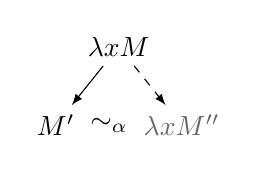
\begin{tikzpicture}[>=latex]
   \node (a) at (2,2) {$\lam x M$};
   \node (b) at (1.2,1) {$M'$};
   \node[opacity=0.6] (d) at (2.8,1) {$\lam x M''$};

   \draw [->] (a) -- (b) ;
   \draw [dashed,->] (a) -- (d) ;
   \path (b) --node{$\alpsym$} (d);
\end{tikzpicture}
\end{minipage}
\begin{minipage}{0.4\textwidth}
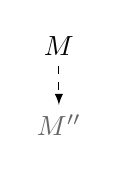
\begin{tikzpicture}[>=latex]
   \node (a) at (2,2) {$M$};
   \node[opacity=0.6] (b) at (2,1) {$M''$};

   \draw [dashed,->] (a) -- (b) ;
\end{tikzpicture}
\end{minipage}
\end{center}
\end{frame}

\begin{frame}
  \begin{lem}[Parallel relation $\beta$-elimination] \
\label{betaelim}

\begin{center}
  \AxiomC{$\lam x M \p \lam y M'\quad N \p N' \quad M' [ y := N' ] \alpsym P$}
  \LeftLabel{\p$\beta$}
  \UnaryInfC{$(\lam x M) N \p P$}
  \DisplayProof
\end{center}  
  \[ \Downarrow \]
  \[ (\exists M'')( \lam x M \p \lam x M'' , M'' [x := N'] \alpsym P) \]

\end{lem} 

\begin{center}
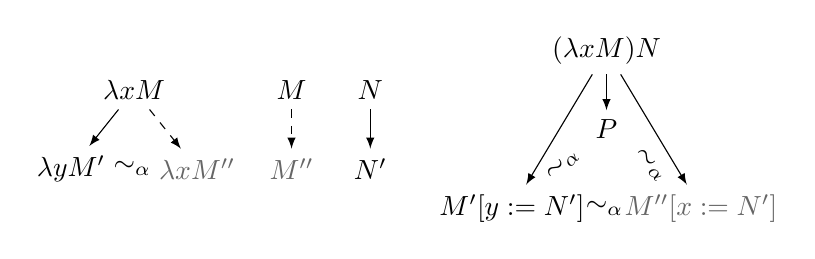
\begin{tikzpicture}[>=latex]
   \node (a) at (2,2) {$\lam x M$};
   \node (b) at (1.2,1) {$\lam y M'$};
   \node[opacity=0.6] (d) at (2.8,1) {$\lam x M''$};

   \node (g) at (4,2) {$M$};
   \node[opacity=0.6] (h) at (4,1) {$M''$};

   \node (e) at (5,2) {$N$};
   \node (f) at (5,1) {$N'$};

   \node (l) at (8,2.5) {$(\lam x M) N$};
   \node (i) at (8,1.5) {$P$};
   \node (j) at (6.8,0.5) {$M'[y:=N']$};
   \node[opacity=0.6] (k) at (9.2,0.5) {$M''[x:=N']$};

   \draw [->] (a) -- (b) ;
   \draw [->] (e) -- (f) ;
   \draw [dashed,->] (g) -- (h) ;
   \draw [dashed,->] (a) -- (d) ;
   \path (b) --node{$\alpsym$} (d);

   \draw [->] (l) -- (i) ;
   \draw [->] (l) -- (j) ;
   \draw [->] (l) -- (k) ;
   \path (i) --node[rotate=45]{$\alpsym$} (j);
   \path (i) --node[rotate=-45]{$\alpsym$} (k);
   \path (j) --node{$\alpsym$} (k);
\end{tikzpicture}
\end{center}
\end{frame}

\begin{frame}



\begin{lem}[Parallel relation substitution lemma]
\label{psubst}
\[ M \p M' \wedge N \p N'  \Rightarrow M [ x := N ] \p M' [ x := N' ] \]
\end{lem}

\begin{itemize}
\item Key lemma for diamond property of \p\ relation.
\item We want to prove it like in pen-and-paper works, for this we need that binders are enough fresh also in the application case, not only in the abstraction case as in previous \alp-induction principles.
\item So we present next \alp-induction principle.
\end{itemize}
\end{frame}

\section{Another Alpha Primitive Induction Principle}

\begin{frame}
\footnotesize{
\begin{minipage}{0.2\linewidth}
  \AxiomC{$\quad$}   \LeftLabel{\ninb v} \UnaryInfC{$x \ninb y$} \DisplayProof
\end{minipage}
\begin{minipage}{0.35\linewidth}
  \AxiomC{$x \ninb M$} 
  \AxiomC{$x \ninb N$}
  \LeftLabel{\ninb a}
  \BinaryInfC{$x \ninb M N$} \DisplayProof
\end{minipage}
\begin{minipage}{0.4\linewidth}
  \AxiomC{$x \neq y$}
  \AxiomC{$x \ninb M$}
  \LeftLabel{\ninb \lam}
  \BinaryInfC{$x  \ninb  \lambda y M$} \DisplayProof
\end{minipage}}

\vspace{2mm}

If for some predicate $P$\ over terms  exists a finite set of atoms $A$\ then:

\footnotesize{
\[ \left.
  \begin{array}{lc}
    P\ \alpha\text{-compatible} & \wedge \\
    \forall a, P(a) & \wedge\\
    \forall M\ N, (\forall b \in A, b \ninb M N) \wedge P(M) \wedge P(N)  \Rightarrow P (M N) & \wedge \\    
    \forall M\ a,\ (\forall b \in A, b \ninb \lam a M) \wedge P(M)   \Rightarrow P (\lam a M) \\    
  \end{array} \right\} \Rightarrow \forall M, P(M)
\]}

\vspace{2mm}
As in Barendregt convention, this induction principle enable us to assume binders position fresh enough from a given finite context of variables $A$ through the entire term induction (not only in the abstraction case). 
  
\end{frame}

\begin{frame}
\begin{lem}[Parallel relation substitution lemma]
\label{psubst}
\[ M \p M' \wedge N \p N'  \Rightarrow M [ x := N ] \p M' [ x := N' ] \]
\end{lem}

\begin{proof}
  Uses previously introduced \alp\ induction principle over $M$\ term. Given some $N,N'$\ terms such that $N \p N'$ , and $x$\ atom, we define the following predicate over terms:

\[ P(M) \equiv \forall M', M \p M' \Rightarrow M [ x := N ] \p M' [ x := N' ] \]

  Next we prove that $P$ is \alp-compatible:  $P(M) \wedge M \alpsym N \Rightarrow P(N)$. 

\scriptsize{  
  \AxiomC{$M \alpsym N$} 
  \AxiomC{$N \p M'$} 
  \LeftLabel{lem.~\ref{pleftalpha}}
  \BinaryInfC{$M \p M'$}
  \AxiomC{$N \p N'$} 
  \LeftLabel{P(M)}
  \BinaryInfC{$M [ x := N ] \p M' [ x := N' ]$}
  \AxiomC{$M \alpsym N$} 
  \LeftLabel{subst.lemma}
  \UnaryInfC{$M [ x := N ] \equiv N [ x := N ]$}
  \LeftLabel{congruence}
  \BinaryInfC{$N [ x := N ] \p M' [ x := N' ]$}
  \DisplayProof}

\end{proof}

 We take as $\{x \} \cup fv(N) \cup fv(N')$\ the set of binders to avoid in the \alp-induction.

\end{frame}

\begin{frame}

  \begin{itemize}
    \item[app. case:]
      \[ \forall P\ Q, (\forall b \in \{x \} \cup fv(N) \cup fv(N'), b \ninb P Q) \wedge P(P) \wedge P(Q)  \Rightarrow P (P Q) \]
    
      \begin{itemize}
      \item[$\beta$\ subcase:] \

        Hypotheses:
        \begin{minipage}{0.8\linewidth}
          \AxiomC{$\lam y P \p \lam z P'$} 
          \AxiomC{$Q \p Q'$}
          \AxiomC{$ P' [z:=Q'] \alpsym R$}
          \LeftLabel{\p $\beta$}
          \TrinaryInfC{$(\lam y P) Q \p R $} \DisplayProof
        \end{minipage}

        Thesis:
        \begin{minipage}{0.8\linewidth}
          $((\lam y P) Q) [x := N ] \p R [x := N']$
        \end{minipage}

        

\vspace{2mm}
Proof:
\vspace{2mm}

        \AxiomC{$(\lam y P) Q \p R $}
        \LeftLabel{lem.~\ref{betaelim}} 
        \UnaryInfC{$\exists P'', \lam y P \p \lam y P'' \wedge P''[y:=Q'] \alpsym R$} 
        \DisplayProof

\vspace{2mm}
%        As $\forall b \in \{x \} \cup fv(N) \cup fv(N'), b \ninb (\lam y P) Q)$\ we have that $y \not\in \{x\} \cup fv(N)$\ and $y \not\in \{x\} \cup fv(N')$.

        \AxiomC{$\forall b \in \{x \} \cup fv(N) \cup fv(N'), b \ninb (\lam y P) Q$}
        \UnaryInfC{$y \not\in \{x\} \cup fv(N)$}
        \UnaryInfC{$ (\lam y P) [x := N]) \alpsym \lam y (P [x := N]) $}
        \DisplayProof

\vspace{2mm}

        Analog

        \AxiomC{$\forall b \in \{x \} \cup fv(N) \cup fv(N'), b \ninb (\lam y P) Q$}
        \UnaryInfC{$y \not\in \{x\} \cup fv(N')$}
        \UnaryInfC{$ (\lam y P'') [x := N'] \alpsym \lam y (P'' [x := N']) $}
        \DisplayProof
      \end{itemize}
    \end{itemize}
  \end{frame}

  \begin{frame}
    




        %%\BinaryInfC{$\lam y (P [x := N]) \p (\lam y P'') [x := N']$}
        \tiny{
        \AxiomC{$\lam y P \p \lam y P''$}
        \LeftLabel{$P(\lam y P)$}
        \UnaryInfC{$
          \begin{array}{c}
              (\lam y P) [x := N] 
            \p \\
            \begin{array}{c}
             (\lam y P'') [x := N'] \\
            \end{array}
          \end{array}$}
        \UnaryInfC{$
          \begin{array}{c}
            \lam y (P [x := N])  \p \\ \lam y (P'' [x := N'])
          \end{array}$}
        \AxiomC{$Q \p Q'$}
        \LeftLabel{$P(Q)$}
        \UnaryInfC{$
          \begin{array}{c}
            Q [x := N]  \p \\ Q' [x := N']
          \end{array}$}
        \AxiomC{$y \not\in \{x\} \cup fv(N')$}
        \UnaryInfC{$
          \begin{array}{c}
            P'' [x := N'] [y := Q' [x := N']] \alpsym \\
            P'' [y := Q' ][x := N']  \equiv  \\
            R [x := N']
          \end{array}$}
        \LeftLabel{$\p\beta$}
        \TrinaryInfC{$\underbrace{(\lam y (P [x := N])) (Q [x := N])}_{\alpsym ((\lam y P) Q) [x := N ]} \p  R [x := N']$}
        \DisplayProof}       

\vspace{10mm}

\begin{center}
        \AxiomC{$ (\lam y P) [x := N]) \alpsym \lam y (P [x := N]) $}
        \AxiomC{$Q [x:=N] \alpsym Q [x:=N]$}
        \LeftLabel{$\alpsym$a}
        \BinaryInfC{($(\lam y P) [x := N]) (Q [x:=N]) \alpsym (\lam y (P [x := N])) (Q [x:=N])$ }
        \UnaryInfC{$((\lam y P) Q) [x:=N] \alpsym (\lam y (P [x := N])) (Q [x:=N])$ }
        \DisplayProof
\end{center}

\end{frame}


\begin{frame}
  \begin{itemize}
    \item[\lam\ case:] $\forall M\ a,\ (\forall b \in \{x \} \cup fv(N) \cup fv(N'), b \ninb \lam a M) \wedge P M   \Rightarrow P (\lam a M) $

        \begin{minipage}{0.4\linewidth}
          Hypotheses: $\lam y P \p Q $
        \end{minipage}
        \begin{minipage}{0.6\linewidth}
          Thesis: $(\lam y P) [x := N ] \p Q [x := N']$
        \end{minipage}

\vspace{2mm}

Proof:


\vspace{2mm}

        \AxiomC{$(\lam y P) \p Q $}
        \LeftLabel{lem.~\ref{lamelim}} 
        \UnaryInfC{$\exists Q', P \p Q' \wedge \lam y P \p \lam y Q' \wedge Q \alpsym \lam y Q'$} 
        \DisplayProof

\vspace{2mm}
\begin{changemargin}{-30px}{0px}
\tiny{
        \AxiomC{$y \not\in \{x\} \cup fv(N)$}         
        \UnaryInfC{$(\lam y P) [x:=N] \alpsym \lam y (P [x:=N])$}
        \AxiomC{$P \p Q' $}         
        \LeftLabel{$P(P)$}         
        \UnaryInfC{$P [x:=N] \p Q' [x:=N']$}
        \UnaryInfC{$\lam y (P [x:=N]) \p \lam y (Q' [x:=N'])$}
        \BinaryInfC{$(\lam y P) [x:=N] \p \lam y (Q' [x:=N'])$}
        \AxiomC{$y \not\in \{x\} \cup fv(N')$}         
        \UnaryInfC{$
          \begin{array}{c}
            \lam y (Q' [x:=N']) \alpsym \\ (\lam y Q') [x:=N']
          \end{array}$}
        \BinaryInfC{$(\lam y P) [x:=N] \p \underbrace{(\lam y Q') [x:=N']}_{\equiv Q[x:=N']\ \text{as}\ Q \alpsym \lam y Q'}$}
        \DisplayProof }
\end{changemargin}
\end{itemize}
\end{frame}

\begin{frame}

  \begin{lem}[Diamond property of parallel relation]
    \label{pdiamond}
    \begin{minipage}{0.7\linewidth}
    $ M \p N \wedge M \p P \Rightarrow \exists Q, N \p Q \wedge P \p      Q $  
    \end{minipage}
    \begin{minipage}{0.2\linewidth}
    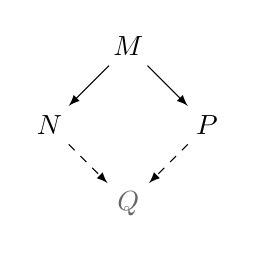
\begin{tikzpicture}[>=latex]  
   \node (a) at (2,2) {$M$};
   \node (b) at (1,1) {$N$};
   \node (c) at (3,1) {$P$};
   \node[opacity=0.6] (d) at (2,0) {$Q$};

   \draw [->] (a) -- (b) ;
   \draw [->] (a) -- (c) ;
   \draw [dashed,->] (b) -- (d) ;
   \draw [dashed,->] (c) -- (d) ;
 \end{tikzpicture}
\end{minipage}
  
  \end{lem}

\begin{proof}
  Induction on the $M$\ term.
\end{proof}
\end{frame}

\begin{frame}

\begin{proof}[\p a-\p $\beta$\ subcase:] 
      Hypotheses:                 
        \begin{minipage}{0.5\linewidth}
          \AxiomC{$\lam x M \p N'$} \AxiomC{$M' \p N''$} \LeftLabel{\p a}
          \BinaryInfC{$(\lam x M) M' \p  N' N''$} \DisplayProof
        \end{minipage}

        \begin{minipage}{0.8\linewidth}
          \AxiomC{$\lam x M \p \lam y P'$} 
          \AxiomC{$M' \p P''$}
          \AxiomC{$ P' [y:=P''] \alpsym P$}
          \LeftLabel{\p $\beta$}
          \TrinaryInfC{$(\lam x M) M' \p P $} \DisplayProof
        \end{minipage}

        Thesis:
        \begin{minipage}{0.5\linewidth}
          $\exists Q, N' N'' \p Q \wedge P \p Q$
        \end{minipage}

\vspace{2mm}
        Proof:
\vspace{2mm}

        Applying eliminations:
\vspace{2mm}
        \AxiomC{$\lam x M \p N' $}
        \LeftLabel{lem.~\ref{lamelim}} 
        \UnaryInfC{$\exists N''', M \p N''' \wedge \lam x M \p \lam x N''' \wedge  N' \alpsym \lam x N'''$}
        \DisplayProof
\vspace{2mm}
        \AxiomC{$(\lam x M) M' \p P $}
        \LeftLabel{lem.~\ref{betaelim}} 
        \UnaryInfC{$\exists P''', \lam x M \p \lam x P''' \wedge P'''[x:=P''] \alpsym P$} 
        \DisplayProof
\end{proof}
\end{frame}

\begin{frame}

        Applying inductive hypothesis and \lam\ elimination.

\vspace{2mm}

\begin{minipage}{0.6\linewidth}
          \AxiomC{$\lam x M \p \lam x N'''$}
          \AxiomC{$\lam x M \p \lam x P'''$} \LeftLabel{ih}
          \BinaryInfC{$\exists Q, \lam x N''' \p \lam x Q \wedge \lam x P''' \p \lam x Q$}
          \DisplayProof
\end{minipage}
\begin{minipage}{0.3\linewidth}
          \AxiomC{$M' \p N''$}
          \AxiomC{$M' \p P''$} \LeftLabel{ih}
          \BinaryInfC{$\exists R, N'' \p R \wedge P'' \p R$}
          \DisplayProof
 \end{minipage}

\vspace{4mm}

        Finally $\exists Q [x:=R], N' N'' \p Q [x:=R] \wedge P \p Q [x:=R]$ as proved next.

\vspace{4mm}


        \AxiomC{$N' \alpsym \lam x N'''$}
        \AxiomC{$N'' \alpsym N''$}
        \LeftLabel{\p a} 
        \BinaryInfC{$N' N'' \alpsym (\lam x N''') N''$}
        \AxiomC{$\lam x N''' \p \lam x S'$}
        \AxiomC{$N'' \p R$}
        \LeftLabel{\p $\beta$} 
        \BinaryInfC{$(\lam x N''') N'' \p Q [x:=R]$}
        \LeftLabel{lem.} 
        \BinaryInfC{$N' N'' \p Q[x:=R]$}
        \DisplayProof

\vspace{4mm}

        \AxiomC{$P \alpsym P'''[x:=P'']$}        
        \AxiomC{$P''' \p Q$}
        \AxiomC{$P'' \p R$}
        \LeftLabel{lemma~\ref{psubst}}
        \BinaryInfC{$P'''[x:=P''] \p Q[x:=R] $}
        \BinaryInfC{$P \p Q[x:=R] $}
        \DisplayProof

\end{frame}


\begin{frame}
\begin{proof}[\lam\ case:] 

        \begin{minipage}{0.8\linewidth}
          Hypotheses: $\lam y M \p N \wedge \lam y M \p P$
        \end{minipage}

        \begin{minipage}{0.8\linewidth}
          Thesis: $\exists Q, N \p Q \wedge P \p Q$
        \end{minipage}


\vspace{2mm}
        Proof:
\vspace{2mm}

        \AxiomC{$(\lam y M) \p N $}
        \LeftLabel{lem.~\ref{lamelim}} 
        \UnaryInfC{$\exists N', M \p N' \wedge  N \alpsym \lam y N'$}


        \AxiomC{$(\lam y M) \p P $}
        \LeftLabel{lem.~\ref{lamelim}} 
        \UnaryInfC{$\exists P', M \p P' \wedge  P \alpsym \lam y P'$}
        \LeftLabel{ih} 
        \BinaryInfC{$\exists Q, N' \p Q \wedge P' \p Q$}
        \UnaryInfC{$\exists \lam y Q,\lam y N' \p \lam y Q \wedge \lam y P' \p \lam y Q$}
        \LeftLabel{lem.\ref{pleftalpha}($ \begin{array}{c}N \alpsym \lam y N' \\ P \alpsym \lam y P' \end{array} $) } 
        \UnaryInfC{$\exists \lam y Q,N \p \lam y Q \wedge P \p \lam y Q$}
        \DisplayProof
      \end{proof}
\end{frame}

\end{document}